\chapter{Results}
\label{chap:results}

This chapter presents the results of the experiments in a way that will facilitate their comparison in the following chapter.

\section{Choosing Resizing Ratio}

\begin{figure}[H]
  \centering
  \includegraphics[width=.7\textwidth]{figures/results/Resizing.png}
  \caption{Speedup and timing w.r.t resizing ratio.}
  \label{fig:resizing-speedup}
\end{figure}

The graph describes the effects of resizing the input images on the total execution time of the pipeline. The horizontal axis represents the resizing ratio applied to the pipeline. It describes the size of the images fed into the pipeline with respect to the raw frame. There are two vertical axes: one to describe the speedup\ref{sec:speedup} and that represents the total execution time in seconds.

Both pipelines tend to get faster with smaller resizing ratios, although the speedup appears to increase at a faster rate for the Fourier-Mellin Pipeline. There is an interesting dip at \(R = 0.75\) for both pipelines which will be discussed further in the next section. 

The Raw Polar Pipeline starts out at around half the execution time of the Fourier-Mellin Pipeline, but as the resizing ratio gets smaller the Fourier-Mellin Pipeline overtakes it. The pipelines seem to break even at around \(R = 0.50\). At \(R = 0.10\) the Fourier-Mellin Pipeline is close to half the execution time of its counterpart.

The pipeline execution time referred to here is the average of a pipeline's runtime for each registration between two frames.

\section{Rotation Estimation}

Based on the previous results and to minimize the execution time necessary to run these tests, the following results are based on running the pipelines using a resizing ratio of 0.10.

\subsection{Fourier-Mellin Pipeline}

\begin{figure}[H]
  \centering
  \includegraphics[width=0.9\textwidth]{figures/results/Rotation-Graphs/FMT-1.png}
  \caption{Results from running the Fourier-Mellin Pipeline with 1º intervals}
  \label{fig:fmresults-skip-0}
\end{figure}

The graph describes the registration results from running the pipeline on simulated frames with a 1º rotation interval between them. Since the input frames represent a rotation of 180º on a section of the reference image \autoref{fig:test_reference}, the horizontal axis represents this rotational movement. There are two vertical axes: one for the rotation delta between frames and the other for the registration error from \autoref{lst:pipeline-phase-correlation}, an indication of confidence in the measurement. The yellow horizontal line represents the actual rotational movement that should be predicted by the pipeline; in this case 1º. As the blue dots come closer to the yellow line the prediction is more accurate. 

The following graphs repeat the experiment using bigger rotation intervals:

\begin{figure}[H]
  \centering
  \includegraphics[width=0.9\textwidth]{figures/results/Rotation-Graphs/FMT-5.png}
  \caption{Results from running the Fourier-Mellin Pipeline with 5º intervals}
\end{figure}

\begin{figure}[H]
  \centering
  \includegraphics[width=0.9\textwidth]{figures/results/Rotation-Graphs/FMT-10.png}
  \caption{Results from running the Fourier-Mellin Pipeline with 10º intervals}
\end{figure}

The Fourier-Mellin Pipeline in all 3 cases struggled to estimate angles correctly at the beginning and the end of the test set frames. This coincides with frames that extend beyond the edge of the source image and are partially missing information. Counter-intuitively the registration error over these measurements is the lowest, showing a higher degree of confidence when compared to the measurements that were actually closest to the reference value. This is visible in the output \autoref{fig:fmtmosaic}, which is the sharpest in the middle where the registrations were closest to the true value, and blurry around the start and end of the semicircle.

\begin{table}[H]
    \centering
    \begin{tabular}{|c|c|c|c|}
        \hline
        \textbf{Parameter} & \textbf{1º} & \textbf{5º} & \textbf{10º} \\ \hline
        Sum & 166.35º & 185.88º & 187.64º \\ \hline
        Average & 0.92º & 5.16º & 10.42º \\ \hline
        StdDev & 0.06º & 0.29º & 0.63º \\ \hline
        StdDev/Average & 7\% & 6\% & 6\% \\ \hline
        Max & 1.05º & 5.52º & 11.05º \\ \hline
        Min & 0.70º & 4.47º & 8.94º \\ \hline
        |Interval - Avg.| & 0.07º & 0.16º & 0.42º \\ \hline
        |Interval - Avg.|/Avg. & 8\% & 3\% & 4\% \\ \hline
    \end{tabular}
    \caption{FMT Pipeline Results}
\end{table}

The table suggests that the pipeline performs similarly for distant rotation estimations. It constantly scores a low StdDev which suggests good precision and consistent registrations. The distance from the estimated interval to the actual value increases with the interval, however, this value remains at sub-degree precision which suggests robustness against the size of the interval. The last metric |Interval - Avg|/Avg suggests that the most precise registration was achieved for the 5º intervals.

The following are the resulting mosaics from these 3 examples:

\begin{figure}[H]
    \centering
    \begin{subfigure}[b]{.48\textwidth}
        \centering
        \includegraphics[height=\textwidth]{figures/results/Rotation-Combined/FMT-1.png}
        \caption{1º Rotations}
    \end{subfigure}
    \hfill
    \begin{subfigure}[b]{.48\textwidth}
        \centering
        \includegraphics[height=\textwidth]{figures/results/Rotation-Combined/FMT-5.png}
        \caption{5º Rotations}
    \end{subfigure}
    \hfill
    \begin{subfigure}[b]{.48\textwidth}
        \centering
        \includegraphics[height=\textwidth]{figures/results/Rotation-Combined/FMT-10.png}
        \caption{10º Rotations}
    \end{subfigure}
    \hfill
    \caption{Mosaics from running the Fourier-Mellin Pipeline with different intervals.}
    \label{fig:fmtmosaic}
\end{figure}


\subsection{Raw Polar Pipeline}

Similar to the previous section, the following graphs describe the registration results from running the pipeline on simulated frames with 1º, 5º and 10º rotational intervals between them:

\begin{figure}[H]
  \centering
  \includegraphics[width=0.9\textwidth]{figures/results/Rotation-Graphs/PC-1.png}
  \caption{Results from running Raw Polar Pipeline with 1º intervals}
\end{figure}

\begin{figure}[H]
  \centering
  \includegraphics[width=0.9\textwidth]{figures/results/Rotation-Graphs/PC-5.png}
  \caption{Results from running Raw Polar Pipeline with 5º intervals}
\end{figure}

\begin{figure}[H]
  \centering
  \includegraphics[width=0.9\textwidth]{figures/results/Rotation-Graphs/PC-10.png}
  \caption{Results from running Raw Polar Pipeline with 10º intervals}
\end{figure}

The Raw Polar Pipeline performed great in all 3 cases with estimated rotation values very close to the reference. The images in \autoref{fig:pcmosaic} are visibly sharper than their \autoref{fig:fmtmosaic} Fourier-Mellin counterparts. The following table corroborates the near-perfect accuracy of the method on pure rotation:

\begin{table}[H]
    \centering
    \begin{tabular}{|c|c|c|c|}
        \hline
        \textbf{Parameter} & \textbf{1º} & \textbf{5º} & \textbf{10º} \\ \hline
        Sum & 186.06 & 179.31 & 179.15 \\ \hline
        Average & 1.03 & 4.98 & 9.95 \\ \hline
        StdDev & 0.03 & 0.04 & 0.08 \\ \hline
        StdDev/Average & 4\% & 1\% & 1\% \\ \hline
        Max & 1.05 & 5.03 & 10.07 \\ \hline
        Min & 0.97 & 4.87 & 9.83 \\ \hline
        |Interval - Avg.| & 0.03 & 0.01 & 0.04 \\ \hline
        |Interval - Avg.|/Avg. & 3\% & 0\% & 0\% \\ \hline
    \end{tabular}
    \caption{Raw Polar Pipeline Results}
\end{table}

The table suggests that the pipeline performs similarly for distant rotation estimations. It constantly scores a low StdDev which suggests good precision and consistent registrations. The distance from the estimated interval to the actual value remains at sub-tenth-of-a-degree precision, which suggests robustness against the size of the interval. The last metric |Interval - Avg|/Avg combined with the Sum suggests that the most precise registration was achieved for the 5º intervals.

The following are the resulting mosaics from these 3 examples:

\begin{figure}[H]
    \centering
    \begin{subfigure}[b]{.48\textwidth}
        \centering
        \includegraphics[height=\textwidth]{figures/results/Rotation-Combined/PC-1.png}
        \caption{1º Rotations.}
    \end{subfigure}
    \hfill
    \begin{subfigure}[b]{.48\textwidth}
        \centering
        \includegraphics[height=\textwidth]{figures/results/Rotation-Combined/PC-5.png}
        \caption{5º Rotations.}
    \end{subfigure}
    \hfill
    \begin{subfigure}[b]{.48\textwidth}
        \centering
        \includegraphics[height=\textwidth]{figures/results/Rotation-Combined/PC-10.png}
        \caption{10º Rotations.}
    \end{subfigure}
    \hfill
    \caption{Mosaics from running the Raw Polar Pipeline with different rotation intervals.}
    \label{fig:pcmosaic}
\end{figure}

\section{Translation Estimation (Sway)}

This section will evaluate the performance of the pipelines when performing sideways translations on the drone, as in left or right sway.

\subsection{Fourier-Mellin Pipeline}

\begin{figure}[H]
  \centering
  \includegraphics[width=0.9\textwidth]{figures/results/Translation-Graph/FMT-0.png}
  \caption{Results from running the Fourier-Mellin Pipeline with 10 px sway intervals.}
\end{figure}

The graph describes the registration results from running the pipeline on simulated frames with a 10 px translation interval along the horizontal axis. It is very similar to the graphs described in the previous section. Since 100 frames were used, the expected translation is 1000px: to simplify the test, the range of this simulated sonar was set so that \(1m = 1px\). 

There are two vertical axes: one for the translation delta along the horizontal axis between frames and the other for the registration error from \autoref{lst:pipeline-phase-correlation}, an indication of confidence in the measurement. The yellow horizontal line represents the actual translation movement that should be predicted by the pipeline; in this case 10 m. The blue line represents the average of the estimated translations. As the blue line comes closer to the yellow line the prediction is more accurate. The following graphs repeat the experiment using bigger translation intervals:


\begin{figure}[H]
    \begin{subfigure}[b]{\textwidth}
        \centering
        \includegraphics[width=0.9\textwidth]{figures/results/Translation-Graph/FMT-4.png}
        \caption{50 m Translation.}
    \end{subfigure}
    \hfill
    \begin{subfigure}[b]{\textwidth}
        \centering
        \includegraphics[width=0.9\textwidth]{figures/results/Translation-Graph/FMT-9.png}
        \caption{100 m Translation.}
    \end{subfigure}
    \hfill
    \caption{Results from running the Fourier-Mellin Pipeline with different sway translation intervals.}
\end{figure}

In all 3 cases, the Fourier-Mellin pipeline appears to be performing extraordinarily well. The average translation seems to be very close to the reference. A quick inspection of the mosaics in \autoref{fig:fmtranslationmosaic} shows that they appear to have been formed correctly, keeping the image sharp. The following table corroborates these observations:


\begin{table}[H]
    \centering
    \begin{tabular}{|c|c|c|c|}
        \hline
        \textbf{Parameter} & \textbf{10 m} & \textbf{50 m} & \textbf{100 m} \\ \hline
        \(\Delta x\) Sum & 1040.42 & 1042.05 & 1050.32 \\ \hline
        \(\Delta x\) Average & 10.40 & 52.10 & 105.03 \\ \hline
        \(\Delta x\) StdDev & 1.68 & 3.85 & 8.86 \\ \hline
        \(\Delta x\) StdDev/Average & 16\% & 7\% & 8\% \\ \hline
        \(\Delta x\) Max & 15.02 & 59.48 & 118.42 \\ \hline
        \(\Delta x\) Min & 7.03 & 46.88 & 92.28 \\ \hline
        \(\Delta x\) |Interval - Avg.| & 0.40 & 2.10 & 5.03 \\ \hline
        \(\Delta x\) |Interval - Avg.|/Avg. & 4\% & 4\% & 5\% \\ \hline
        \(\Delta\Theta\) Sum & 2.47 & 2.47 & 2.82 \\ \hline
    \end{tabular}
    \caption{Raw Polar Pipeline Results.}
\end{table}

The pipeline performs consistently for all three cases. While the standard deviation relative to the average (StdDev/Average) is somewhat higher for the 10 m interval at 16\%, it stabilizes for the 50 m and 100 m intervals at 7\% and 8\%, respectively, indicating improved precision at greater distances. There is very little error introduced by erroneous angular estimations \(\Delta\Theta\) and the total error with respect to the average (|Interval - Avg.|/Avg.) is quite low at 4\% to 5\% for all registrations.  


\begin{figure}[H]
    \centering
    \begin{subfigure}[b]{\textwidth}
        \centering
        \includegraphics[width=0.9\textwidth]{figures/results/Translation-Combined/FMT-0.png}
        \caption{10 m Translation.}
    \end{subfigure}
    \hfill
    \begin{subfigure}[b]{\textwidth}
        \centering
        \includegraphics[width=0.9\textwidth]{figures/results/Translation-Combined/FMT-4.png}
        \caption{50 m Translation.}
    \end{subfigure}
    \hfill
    \begin{subfigure}[b]{\textwidth}
        \centering
        \includegraphics[width=0.9\textwidth]{figures/results/Translation-Combined/FMT-9.png}
        \caption{100 m Translation.}
    \end{subfigure}
    \hfill
    \caption{Mosaics from running the Fourier-Mellin Pipeline with different sway intervals.}
    \label{fig:fmtranslationmosaic}
\end{figure}





\subsection{Raw Polar Pipeline}
\label{sec:sway-hurtos}

\begin{figure}[H]
  \centering
  \includegraphics[width=0.9\textwidth]{figures/results/Translation-Graph/PC-0.png}
  \caption{Results from running the Raw Polar Pipeline with 10 px sway intervals.}
\end{figure}

The results from the Raw Polar Pipeline on translation along were quite underwhelming. The estimation is off, and there is a rotation component that scrambles the mosaic. 

\begin{figure}[H]
  \centering
  \includegraphics[width=.7\textwidth]{figures/results/Translation-Combined/PC-0.png}
  \caption{Mosaic from running the Raw Polar Pipeline with 10 px sway intervals.}
  \label{fig:pc-sway-mosaic}
\end{figure}

As can be seen in the table, the error is estimated to be about 80\% of the actual measurement which is not a good sign. Even though there was supposed to be no rotation at all, the pipeline estimates a rotation of 192º. This could be an indicator that something went wrong in the estimation of the rotation and in turn affected the translation.

\begin{table}[H]
    \centering
    \begin{tabular}{|c|c|}
        \hline
        \textbf{Parameter} & \textbf{10 m} \\ \hline
        \(\Delta x\) Sum & 4931.47 \\ \hline
        \(\Delta x\) Average & 49.31 \\ \hline
        \(\Delta x\) StdDev & 2.00 \\ \hline
        \(\Delta x\) StdDev/Average & 4\% \\ \hline
        \(\Delta x\) Max & 52.75 \\ \hline
        \(\Delta x\) Min & 44.14 \\ \hline
        \(\Delta x\) |Interval - Avg.| & 39.31 \\ \hline
        \(\Delta x\) |Interval - Avg.|/Avg. & 80\% \\ \hline
        \(\Delta\Theta\) Sum & 192.97 \\ \hline
    \end{tabular}
    \caption{Raw Polar Pipeline Results.}
\end{table}

The table confirms that during the estimation, the pipeline failed to recognize that the total rotation should be 0º. This introduced translation steps that were bigger than expected at an average of 49.31. Although the registrations are very consistent with a low StdDev (4\% of the average), taking a quick look at \autoref{fig:pc-sway-mosaic} shows that it wasn't accurate at all. Since the performance of the pipeline is already terrible at this point, there is little value in repeating the test under more demanding conditions.


\section{Translation Estimation (Surge)}

This section will focus on estimating translations along the surge axis of the drone, as in moving forwards or backward. 

\subsection{Fourier-Mellin Pipeline}

\begin{figure}[H]
  \centering
  \includegraphics[width=0.9\textwidth]{figures/results/Thesis-Surge/FMT-0.png}
  \caption{Results from running the Fourier-Mellin Pipeline with 10 px surge intervals.}
\end{figure}

\begin{figure}[H]
  \centering
  \includegraphics[width=0.9\textwidth]{figures/results/Thesis-Surge/FMT-4.png}
  \caption{Results from running the Fourier-Mellin Pipeline with 50 px surge intervals.}
\end{figure}

\begin{figure}[H]
  \centering
  \includegraphics[width=0.9\textwidth]{figures/results/Thesis-Surge/FMT-9.png}
  \caption{Results from running the Fourier-Mellin Pipeline with 100 px surge intervals.}
\end{figure}

On quick inspection of the graphs, it is evident that the performance of the estimation along the surge axis for the Fourier-Mellin Pipeline is very similar to the sway axis. The averages seem to be close to the reference values even with distant registrations. 

\begin{table}[H]
    \centering
    \begin{tabular}{|c|c|c|c|}
        \hline
        \textbf{Parameter} & \textbf{10 m} & \textbf{50 m} & \textbf{100 m} \\ \hline
        \(\Delta x\) Sum & 911.20 & 895.56 & 1321.60 \\ \hline
        \(\Delta x\) Average & 9.20 & 47.13 & 146.84 \\ \hline
        \(\Delta x\) StdDev & 3.22 & 15.11 & 129.37 \\ \hline
        \(\Delta x\) StdDev/Average & 34.95\% & 32.06\% & 88.10\% \\ \hline
        \(\Delta x\) Max & 15.46 & 80.49 & 474.31 \\ \hline
        \(\Delta x\) Min & 0.95 & 24.88 & 55.88 \\ \hline
        \(\Delta x\) |Interval - Avg.| & 0.80 & 2.87 & 46.84 \\ \hline
        \(\Delta x\) |Interval - Avg.|/Avg. & 8.65\% & 6.08\% & 31.90\% \\ \hline
        \(\Delta\Theta\) Sum & -2.00 & -1.18 & -76.82 \\ \hline
    \end{tabular}
    \caption{Fourier-Mellin Pipeline Results.}
\end{table}

However, upon closer inspection of the metrics, it is evident that there is some degradation of performance, especially for the registration of the most distant frames at 100 m. This is visible in the generated mosaics, where the last one becomes very blurry:

\begin{figure}[H]
    \centering
    \begin{subfigure}[b]{0.47\textwidth}
        \centering
        \includegraphics[width=\textwidth]{figures/results/Translation-Surge-Combined/FMT-0.png}
        \caption{10 px Translation.}
        \label{sfig:fmt-surge-0}
    \end{subfigure}
    \hfill
    \begin{subfigure}[b]{0.47\textwidth}
        \centering
        \includegraphics[width=\textwidth]{figures/results/Translation-Surge-Combined/FMT-4.png}
        \caption{50 px Translation.}
        \label{sfig:fmt-surge-4}
    \end{subfigure}
    \hfill
    \begin{subfigure}[b]{0.47\textwidth}
        \centering
        \includegraphics[width=\textwidth]{figures/results/Translation-Surge-Combined/FMT-9.png}
        \caption{100 px Translation.}
        \label{sfig:fmt-surge-9}
    \end{subfigure}
    \hfill
    \caption{Mosaics from running the Fourier-Mellin Pipeline with different surge intervals.}
\end{figure}

There is a very visible misalignment in \autoref{sfig:fmt-surge-9}. The clearest image comes from the 10 px intervals.

\subsection{Raw Polar Pipeline}
\label{sec:surge-hurtos}

\begin{figure}[H]
  \centering
  \includegraphics[width=0.9\textwidth]{figures/results/Translation-Surge/PC-0.png}
  \caption{Results from running the Raw Polar Pipeline with 10 px surge intervals.}
\end{figure}

\begin{figure}[H]
  \centering
  \includegraphics[width=0.9\textwidth]{figures/results/Translation-Surge/PC-4.png}
  \caption{Results from running the Raw Polar Pipeline with 50 px surge intervals.}
\end{figure}

\begin{figure}[H]
  \centering
  \includegraphics[width=0.9\textwidth]{figures/results/Translation-Surge/PC-9.png}
  \caption{Results from running the Raw Polar Pipeline with 100 px surge intervals.}
\end{figure}


These results are more promising than their equivalent for the Fourier-Mellin Transform as it appears that the average of the estimation is closer to the reference. Not only that, these results are completely different from the ones obtained for translation along the sway axis. To be sure, we refer to the table:

\begin{table}[H]
    \centering
    \begin{tabular}{|c|c|c|c|}
        \hline
        \textbf{Parameter} & \textbf{10 m} & \textbf{50 m} & \textbf{100 m} \\ \hline
        \(\Delta x\) Sum & 981.97 & 920.70 & 910.60 \\ \hline
        \(\Delta x\) Average & 9.92 & 48.46 & 101.18 \\ \hline
        \(\Delta x\) StdDev & 1.96 & 16.61 & 79.95 \\ \hline
        \(\Delta x\) StdDev/Average & 19.72\% & 34.28\% & 79.02\% \\ \hline
        \(\Delta x\) Max & 13.69 & 76.76 & 238.34 \\ \hline
        \(\Delta x\) Min & 5.91 & 20.01 & -16.67 \\ \hline
        \(\Delta x\) |Interval - Avg.| & 0.08 & 1.54 & 1.18 \\ \hline
        \(\Delta x\) |Interval - Avg.|/Avg. & 0.82\% & 3.18\% & 1.16\% \\ \hline
        \(\Delta\Theta\) Sum & 0.75 & -0.23 & 1.95 \\ \hline
    \end{tabular}
    \caption{Raw Polar Pipeline Results.}
\end{table}

It appears that the pipeline is very stable regardless of registration distance. There is almost no influence from unwanted rotations, and the percentual error with respect to the average (|Interval - Avg.|/Avg.) is very low for all 3 cases. Precision is not that great, with high relative standard deviation values (StdDev/Average). The combined graphs, however, speak for themselves:

\begin{figure}[H]
    \centering
    \begin{subfigure}[b]{0.47\textwidth}
        \centering
        \includegraphics[width=\textwidth]{figures/results/Translation-Surge-Combined/PC-0.png}
        \caption{10 px Translation.}
    \end{subfigure}
    \hfill
    \begin{subfigure}[b]{0.47\textwidth}
        \centering
        \includegraphics[width=\textwidth]{figures/results/Translation-Surge-Combined/PC-4.png}
        \caption{50 px Translation.}
    \end{subfigure}
    \hfill
    \begin{subfigure}[b]{0.47\textwidth}
        \centering
        \includegraphics[width=\textwidth]{figures/results/Translation-Surge-Combined/PC-9.png}
        \caption{100 px Translation.}
    \end{subfigure}
    \hfill
    \caption{Mosaics from running the Raw Polar Pipeline with different surge intervals.}
\end{figure}

On visual inspection, the alignment in all 3 cases is good. Again the seams begin to show very clearly on higher translations, achieving the best clarity on the 10 px translations. 


\section{Examples on Sonar Data}

Finally, we get to real-world examples using the drone. In this first example, pure rotation is applied on the left corner of the marina from \autoref{fig:marina}. The rotation is controlled by the pilot to be 180º. Using a resizing ratio of 0.1, the pipelines determined that the range resolution for this image will be 0.12 m/pixel.

Using the outputs of the pipelines and an \href{https://www.utilities-online.info/online-pixel-ruler}{online pixel ruler} the following annotated results were obtained:

\begin{figure}[H]
    \centering
    \begin{subfigure}[b]{0.47\textwidth}
        \centering
        \includegraphics[width=\textwidth]{figures/results/Real/PC-Rotation-Annotated.png}
        \caption{Raw Polar Mosaic.}
    \end{subfigure}
    \hfill
    \begin{subfigure}[b]{0.47\textwidth}
        \centering
        \includegraphics[width=\textwidth]{figures/results/Real/FMT-Rotation-Annotated.png}
        \caption{Fourier-Mellin Mosaic.}
    \end{subfigure}
    \label{fig:sonar-mosaic}
    \caption{Mosaics from running the pipelines on real rotation data.}
\end{figure}

The values appear to be very close to estimates obtained from \href{https://earth.google.com/web/@63.44158505,10.41727398,0.31239001a,140.28884032d,35y,151.00013963h,0t,0r/data=OgMKATA}{Google Earth}: 3.5 m (orange), 21 m (red), 3.5 m (green), 5 m (blue). However, it's difficult to trust these values with absolute certainty, since the measurement was done by virtual ruler.

\begin{table}[H]
    \centering
    \begin{tabular}{|c|c|c|}
        \hline
        \textbf{Parameter} & \textbf{Raw Polar} & \textbf{Fourier-Mellin} \\ \hline
        Sum & 209.40 & 198.11 \\ \hline
        Average & 0.55 & 0.52 \\ \hline
        StdDev & 0.32 & 0.43 \\ \hline
        StdDev/Average & 59\% & 82\% \\ \hline
        Max & 1.86 & 1.87 \\ \hline
        Min & -0.29 & -0.46 \\ \hline    
        \end{tabular}
    \caption{Pipeline results.}
\end{table}

Both pipelines got close to the actual rotation of 180º but were overshot by 16º and 11º respectively. This explains the visual distortion on the outputs, making angles that should be square a little off.   

Although the results are hard to compare, through visual inspection, it seems as though the Raw Polar Pipeline is performing better. We repeat the test on different input, where given a different range setting the pipelines determined that the range resolution for this image will be 0.26 m/pixel.

\begin{figure}[H]
    \centering
    \begin{subfigure}[b]{0.47\textwidth}
        \centering
        \includegraphics[width=\textwidth]{figures/results/Real/Example2/PC-Annotated.png}
        \caption{Raw Polar Mosaic.}
    \end{subfigure}
    \hfill
    \begin{subfigure}[b]{0.47\textwidth}
        \centering
        \includegraphics[width=\textwidth]{figures/results/Real/Example2/FMT-Annotated.png}
        \caption{Fourier-Mellin Mosaic.}
    \end{subfigure}
    \label{fig:sonar-mosaic}
    \caption{Mosaics from running the pipelines on real rotation data.}
\end{figure}


Comparing this data to \href{https://earth.google.com/web/@63.44140267,10.4184834,0.19057254a,140.41066178d,35y,125.00002682h,0t,0r/data=OgMKATA}{Google Earth} the red line should measure approximately 34.6 m and the blue line around 30.8 m. This makes is evident that the Fourier-Mellin Pipeline in not detecting rotations properly. The Raw Polar approach is within 1 m precision for both lines whereas the Fourier-Mellin approach gets in the worst case around 8.5 m error. 


Another interesting result on real data is how mosaicing reduces noise:


\begin{figure}[H]
    \centering
    \begin{subfigure}[b]{0.47\textwidth}
        \centering
        \includegraphics[width=\textwidth]{figures/results/Real/ExampleMosaic/combined_00000001.png}
        \caption{Input Frame.}
    \end{subfigure}
    \hfill
    \begin{subfigure}[b]{0.47\textwidth}
        \centering
        \includegraphics[width=\textwidth]{figures/results/Real/ExampleMosaic/combined.png}
        \caption{Raw Polar Pipeline Mosaic.}
    \end{subfigure}
    \label{fig:sonar-mosaic}
    \caption{Difference in noise between a single frame and mosaic.}
\end{figure}

The overall effect is that the image is less grainy, some of the voids are filled in by data from other frames and it's easier to identify features like the two pillars close to the wall. 